\chapter{Theoretical Framework}
\label{chapter:theoretical-framework}


This chapter describes the theoretical concepts needed to understand the work that will be developed during the research's execution.


\section{FER}

\subsection{Emotional Labeling}

\subsection{FER in-the-wild}

\section{FER Archiquectures}

\subsection{Deep Learning for FER}

\subsection{Visual Transformer}

\section{FER Performance and Evaluation}


\subsection{Performance Metrics for FER}

\subsection{Evaluation of Modified Heads}

\cite{dosovitskiy_image_2021}

%\section{Concept 1}
%
%\label{section:Concept1}
%
%First theoretical framework concept goes here.
%
%\subsection{Subsection of Concept 1} 
%\subsection{Subsection 2 of Concept 1}
%Some text goes here \cite{examplereference}. An example of displaying and referencing an image is shown in \textbf{Figure \ref{fig:example}}
%
%
%\begin{figure}
%	\begin{center}
%		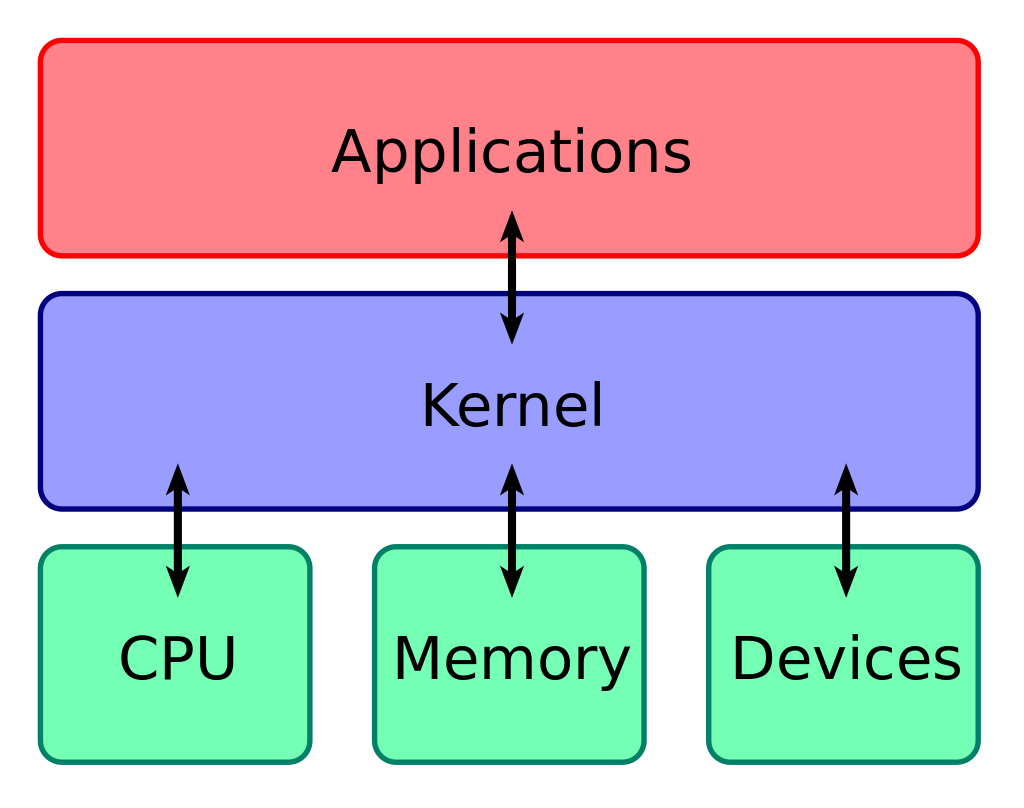
\includegraphics[width=1\columnwidth]{../img/image.png}
%		\caption[]{Example image with reference \cite{examplereference}.}
%		\label{fig:example}
%	\end{center}
%\end{figure}
%
%
%\section{Concept 2}
%
%\label{section:Concept2}
%
%\subsection{Subsection Concept 2}
%
%\subsubsection{Subsection 2 Concept 2}
%
%\section{Concept 3}
%An example of pseudo-code can be seen in \textbf{Algorithm \ref{examplepseudocode}}
%
%\begin{pseudocode}{Pseudo\_Code}{Input} \label{examplepseudocode}
%	\FOR y \GETS 1 \TO Input.MaxL \DO
%	\BEGIN
%	\FOR x \GETS 1 \TO Input.MaxH \DO
%	\BEGIN
%	a \GETS \CALL {FunctionCall}{x,y}\\
%	b \GETS \CALL {AnotherFunction}{x, y}\\
%	\CALL {ThirdFunction}{a,b}
%	\END
%	\END
%\end{pseudocode}
%
%
%\subsection{Example equation}
% Equation \ref{eq:1} shows an example equation.
%
%\[
%I=(L\cdot N) \tag{1} \label{eq:1}
%\]
  
\section{Related Work}
The related work for the research is include in this section:

Facial expression recognition (FER) has been extensively studied over the past decades, evolving from traditional machine learning approaches to deep learning methods. Early FER systems relied on handcrafted features such as Local Binary Patterns (LBP) and Histogram of Oriented Gradients (HOG). These approaches, while computationally efficient, often struggled to generalize across diverse datasets due to limited feature representation capabilities. 

The advent of convolutional neural networks (CNNs) revolutionized FER by enabling automatic feature extraction, with architectures such as VGGNet, ResNet \cite{he_deep_2015}, and EfficientNet achieving significant performance improvements. However, CNNs face limitations in capturing global dependencies and spatial relationships in images, which has motivated the exploration of transformer-based models in computer vision tasks \cite{islam_recent_2023}.

The introduction of Vision Transformers (ViTs) by Dosovitskiy \cite{dosovitskiy_image_2021} marked a significant shift in how visual tasks are approached. By leveraging self-attention mechanisms, ViTs can model long-range dependencies and capture richer contextual information compared to traditional CNNs.

Subsequent works have refined transformer architectures for visual tasks, including pyramid-based models that enhance multi-scale feature representation\cite{zheng_poster_2022}. For FER, transformer-based methods have shown promise by addressing challenges such as subtle facial expression variations and occlusions. Notably, pyramid transformers, such as those used in POSTER, offer hierarchical feature extraction capabilities that are particularly beneficial for FER.



\begin{table}[H]
\centering
\caption{State of the Art of FER systems}
\renewcommand{\arraystretch}{1.5} % Adjust row spacing
\begin{tabular}{llll}
\hline
\textbf{Model}   & \textbf{Accuracy (\%)} & \textbf{Parameters (M)} & \textbf{Key Insights}                                                                                                       \\ \hline
ResNet-50   \cite{he_deep_2015}     & 86.34                  & 24.6 & \begin{tabular}[c]{@{}l@{}}Baseline CNN with strong local \\ feature extraction but lacks \\ global context.\end{tabular}   \\
Swin Transformer \cite{lixu_swin_2021} & 90.97                & 28.3                    & \begin{tabular}[c]{@{}l@{}}Hierarchical ViT with local-global \\ features but computationally \\ expensive.\end{tabular}    \\
ViT (Base)  \cite{dosovitskiy_image_2021}     & 86.34                 & 86.4               & \begin{tabular}[c]{@{}l@{}}Standard transformer struggles \\ with subtle FER cues in \\ real-world conditions.\end{tabular} \\
\textbf{POSTER} \cite{zheng_poster_2022}  & \textbf{92.05}         & \textbf{Not specified}           & \begin{tabular}[c]{@{}l@{}}Combines pyramid attention and \\ cross-fusion for local-global \\ feature synergy.\end{tabular} \\ \hline
\end{tabular}
\end{table}
